\subsubsection{Rancangan Antarmuka}

Rancangan antarmuka digunakan untuk menggambarkan tampilan yang digunakan pengguna pada proses \textit{checkout}. Antarmuka dirancang untuk layar sentuh dan dibagi menjadi tiga tahap, yaitu pindai nampan, verifikasi lauk, serta konfirmasi dan bayar. Tahap yang sedang berlangsung ditunjukkan oleh indikator langkah pada bagian atas setiap tampilan sehingga pengguna mengetahui posisinya dalam alur \textit{checkout}.

Pada tahap pertama, antarmuka menampilkan pratinjau kamera yang mengarah ke area pengambilan citra beserta status kamera. Setelah piring ditempatkan, pengguna menekan tombol \textit{Scan Makanan Sekarang} untuk mengambil citra dan memulai proses pengenalan lauk. Tampilan tahap pertama ditunjukkan pada Gambar~\ref{fig:antarmuka-pindai}.

\begin{figure}[H]
    \centering
    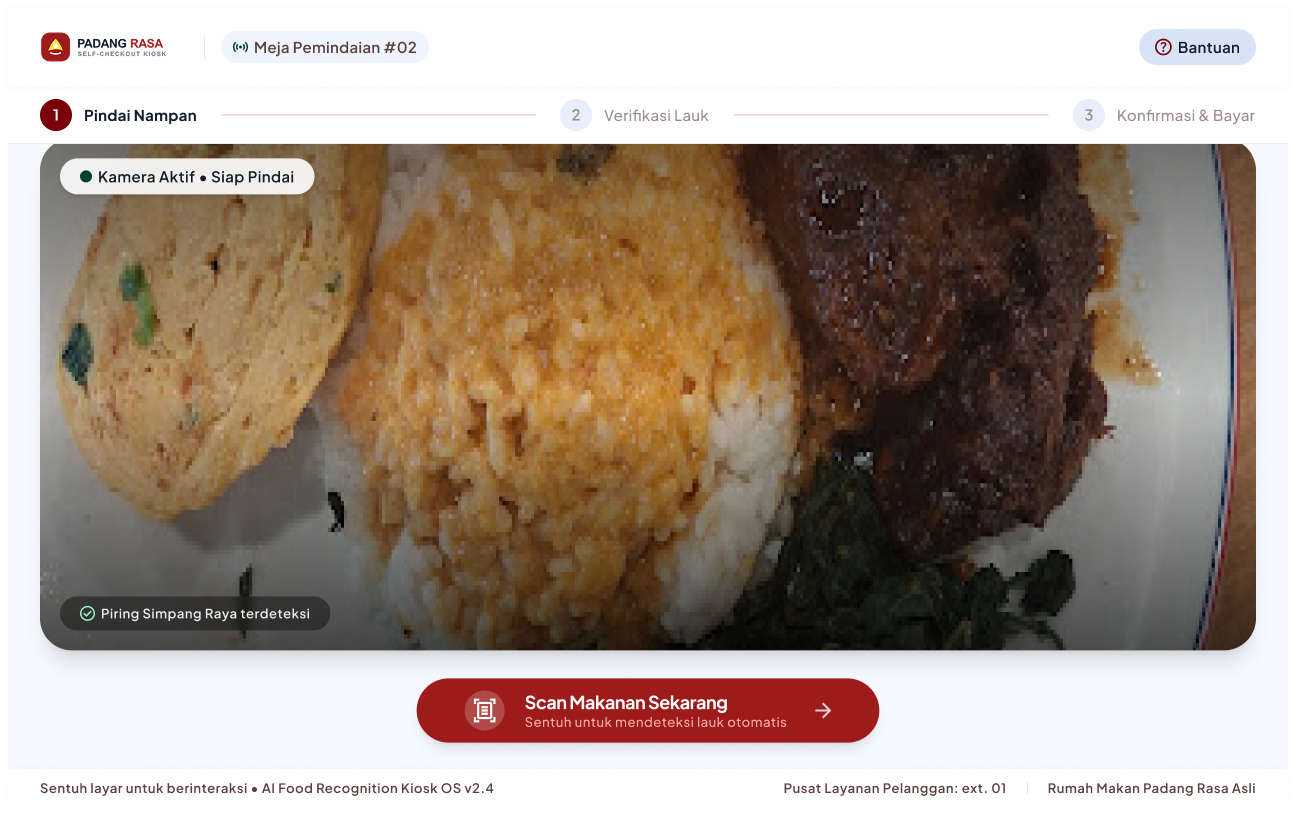
\includegraphics[width=\textwidth]{figures/design/screen_1.png}
    \caption{Rancangan antarmuka tahap pindai nampan}
    \label{fig:antarmuka-pindai}
    \par\smallskip
    {\footnotesize Sumber: Dokumentasi pribadi}
\end{figure}

Pada tahap kedua, bagian kiri menampilkan citra piring yang telah diambil, sedangkan bagian kanan menampilkan hasil pengenalan berupa jenis makanan yang dikenali, harga satuan, jumlah, dan subtotal setiap kelas. Total tagihan ditampilkan pada bagian bawah daftar. Pengguna dapat memeriksa hasil tersebut, menyesuaikan jumlah apabila hasil pengenalan kurang sesuai, atau mengambil citra kembali melalui tombol \textit{Scan Ulang}. Tampilan tahap kedua ditunjukkan pada Gambar~\ref{fig:antarmuka-verifikasi}.

\begin{figure}[H]
    \centering
    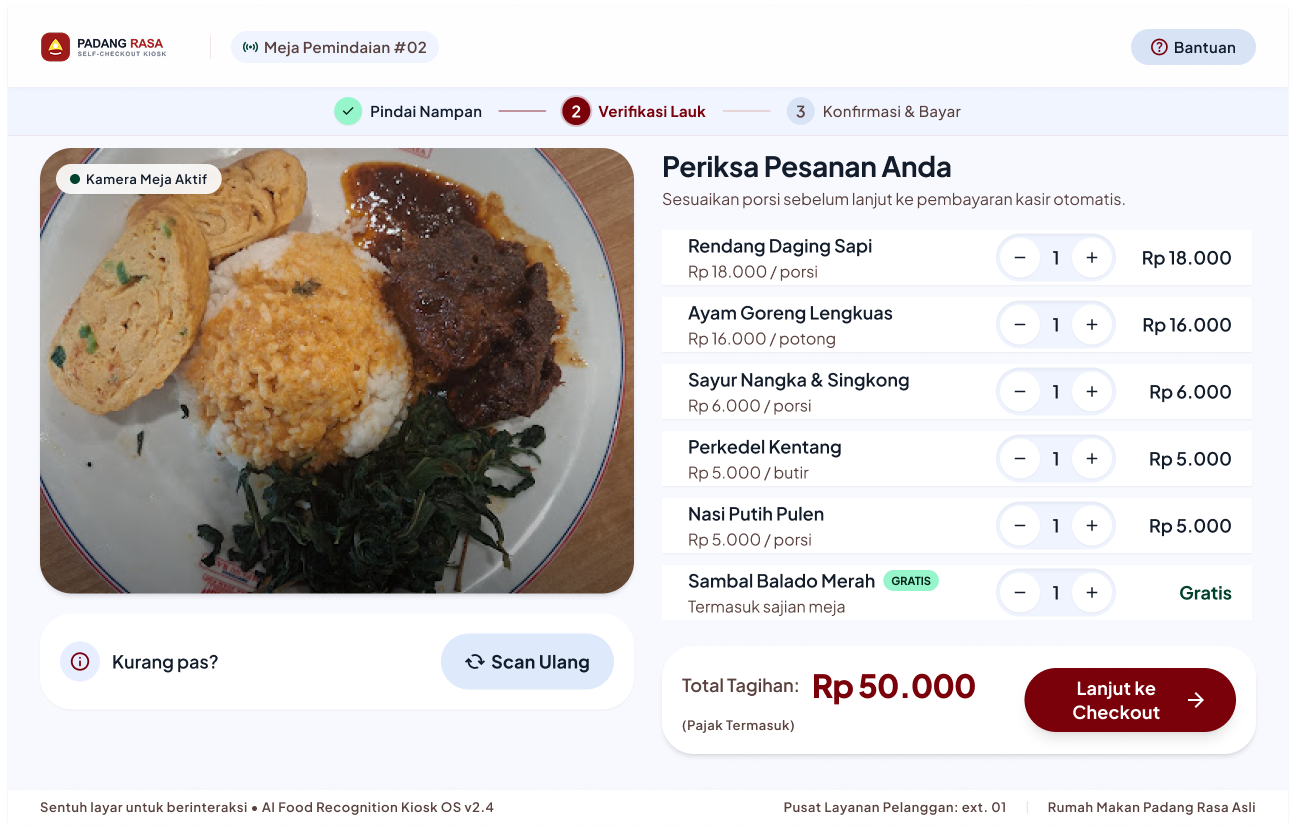
\includegraphics[width=\textwidth]{figures/design/screen_2.png}
    \caption{Rancangan antarmuka tahap verifikasi lauk}
    \label{fig:antarmuka-verifikasi}
    \par\smallskip
    {\footnotesize Sumber: Dokumentasi pribadi}
\end{figure}

Pada tahap ketiga, antarmuka menampilkan ringkasan pesanan yang memuat citra piring, daftar makanan beserta jumlah dan subtotal, serta total pembayaran. Pengguna dapat kembali ke tahap verifikasi melalui tombol \textit{Kembali} atau menyelesaikan proses \textit{checkout} melalui tombol konfirmasi. Proses pembayaran setelah konfirmasi tidak termasuk dalam cakupan sistem. Tampilan tahap ketiga ditunjukkan pada Gambar~\ref{fig:antarmuka-konfirmasi}.

\begin{figure}[H]
    \centering
    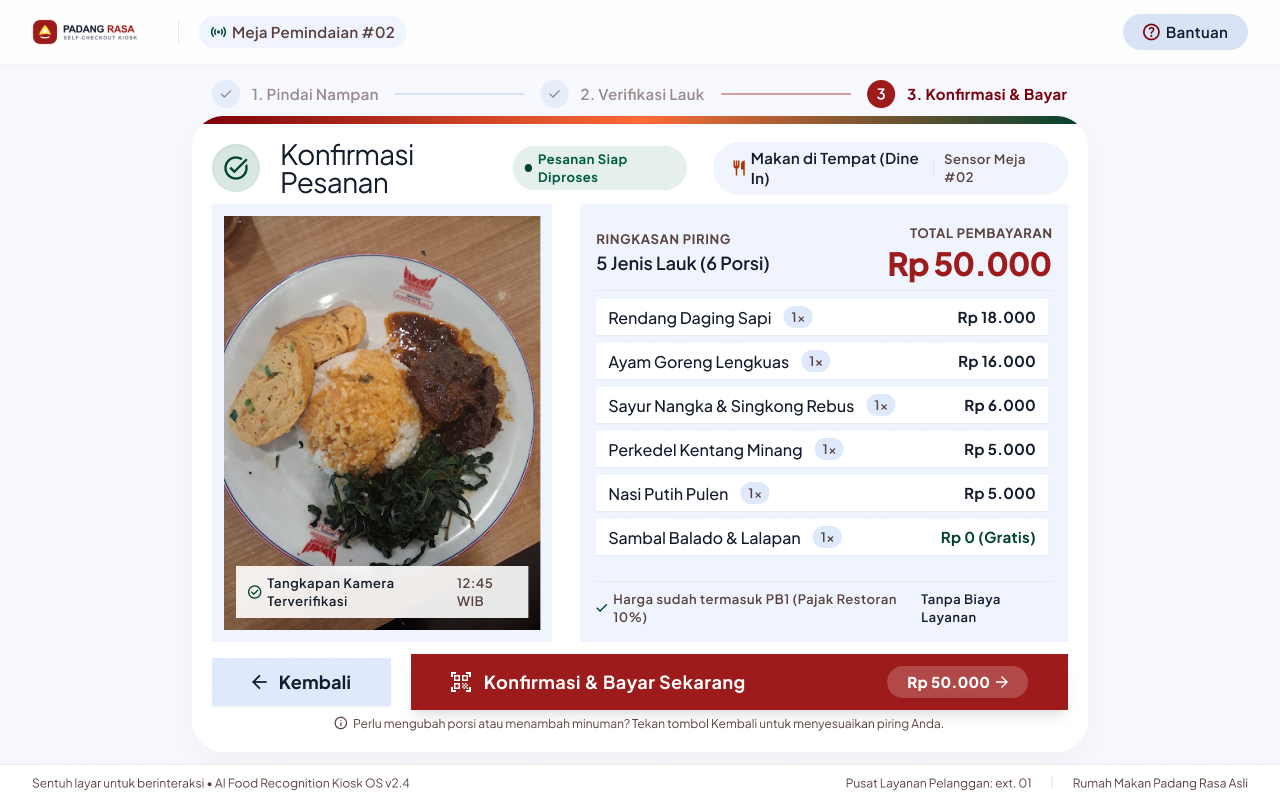
\includegraphics[width=\textwidth]{figures/design/screen_3.png}
    \caption{Rancangan antarmuka tahap konfirmasi dan bayar}
    \label{fig:antarmuka-konfirmasi}
    \par\smallskip
    {\footnotesize Sumber: Dokumentasi pribadi}
\end{figure}
